\documentclass{article}
\usepackage{scribe}
\usepackage{amssymb}
\usepackage{amsmath}

\usepackage{csquotes}
\usepackage{amssymb}


\newtheorem{hw}{Homework Problem}
\newtheorem{ex}{Example}

\newcommand{\Perp}{{\bot\negthickspace\negthickspace\bot}}


%%% Unless you have very specific needs, the lines above should include
%%% all the typesetting features you need.

 


\begin{document}

\begin{lecture}{September 4th, 2019}{Lingfeng Zhang}{300134245}{lzhan278@uottawa.ca}

\section{Course Information (Lecture 00)}
\begin{itemize}
\item Professor: Yongyi Mao
\item Office: SITE 5039
\item Email: ymao@uottawa.ca
\item Office Hour: send email to schedule an appointment(most Monday Morning)
\item Course Prerequisites:
	\begin{itemize}
	\item Mathematics
		\begin{itemize}
		\item Linear Algebra
		\item Calculus
		\item Probability Theory and Statics
		\end{itemize}
	\item Programming Language
		\begin{itemize}
		\item Python
		\end{itemize}
	\item Framework
		\begin{itemize}
		\item Pytorch (Recommended)
		\item TensorFlow
		\end{itemize}
	\item Writing Format
		\begin{itemize}
		\item \LaTeX
		\end{itemize}
	\item Running Platform
		\begin{itemize}
		\item Local
		\item Google Colab (free GPU, running code on the cloud)
		\end{itemize}
	\end{itemize} 
\item Textbook and References
	\begin{enumerate}
	\item No Textbook
	\item Ian Goodfellow, Yoshua Bengio and Aaron Courville, Deep Learning, MIT press, 2016, Electronic version available at \newline \texttt{http://www.deeplearningbook.org}
	\item Richard S. Sutton (Author), Andrew G. Barto, Reinforcement Learning: An Introduction, MIT Press, 1998; the second edition is to appear soon.
	\end{enumerate}
	\item Grading Scheme
	
\begin{center}Project-Augmented Exam-Gated Homeworks\end{center}
\begin{eqnarray}
Grade = HomeworkGrade\times WrittenExamGrade+ProjectGrade+ScribeBonus\end{eqnarray}
\begin{eqnarray}
Grade  \leqslant 110\%
\end{eqnarray}
\end{itemize} 

\begin{enumerate}
\item HomeworkGrade worth  60\% and the maximum members of each homework group is 2.
\item WrittenExamGrade is the any number between 0 and 1,like the weight of HomeworkGrade. The content of this  exam is related to the homework, making sure you have grasped the idea of your finished homework totally.
\item ProjectGrade worth 40\% and the maximum members of each project group is 6. To choose the topic of project, it follows first-come-first-pick basis. There is extra 5\% bonus about project presentation on the research plan(scheduled at some out-of-class slots) .
\item ScribeBonus worth up to 5\%. Students can submit well-formatted PDF version lecture scripts by using \LaTeX ,each of which is awarded up to 1\%. Maximum number of scripts for each lecture is 3(first come first grab in UO brightspace's Discussion module).
\end{enumerate}


\section{Machine Learning Basis (Lecture 01)}

Deep Learning $\neq$ Machine Learning $\neq$  Artificial Intelligence

\textbf{Definition by Tom M. Mitchell}
\begin{displayquote}A computer program is said to learn from experience E with respect to some class of tasks T and performance measure P if its performance at tasks in T, as measured by P, improves with experience E.
\end{displayquote}

task $:=$ input/output specificatoin

\textbf{Application in ML}
\begin{itemize}
\item Predicting stock prices
\item Loan application
\item Discovering lung cancers
\item Playing chess
\item ect... 
\end{itemize}

\textbf{Main Classes of ML Problems}
\begin{enumerate}
\item Supervised Learning
	\begin{enumerate}
	\item training set, testing set
	\item with target
	\item Examples
		\begin{enumerate}
		\item Regression
		\item Classification
		\end{enumerate}
	\end{enumerate}
\item Unsupervised Learning
	\begin{enumerate}
	\item find structure in dataset
	\item Examples
		\begin{enumerate}
		\item Clustering
		\item Density Estimation, like DBSCAN Algorithm
		\end{enumerate}
	\end{enumerate}
\item Reinforcement Learning
	\begin{enumerate}
	\item Gaining more rewards by changing "state"
	\item Example: Chess-Playing program (Alpha Go)
	\end{enumerate}
\end{enumerate}

\textbf{Model: $\mathcal{H}$ of hypothesis}
\begin{enumerate}
\item Parametric models: with fixed number of parameters(initialized manually sometimes), independent of sample size
\item Non-Parametric models
\end{enumerate}

\textbf{Loss Functions: $\mathcal{L}(\theta)$}

\begin{itemize}
\item $\theta$ represents model parameters in space $\Theta$
\item one-to-one correspondence: $\Theta\Longleftrightarrow\mathcal{H}$
\item measures \textit{error}
\item learning is to reduce \textit{error}
\end{itemize}
\begin{eqnarray}
\hat\theta:=arg\min\limits_{\theta\in\Theta}\mathcal{L}(\theta)
\end{eqnarray}
In this equation, $arg$ represents $\theta$ values when $\mathcal{L}(\theta)$ reaches the minimum
\begin{ex}
\textbf{Regression}

X takes value in $\mathbb{R}^K$ $\Rightarrow$ K kinds of features

\begin{eqnarray}
Y \approx f(X;\theta)
\end{eqnarray}

\textbf{Linear Regression Model}
\begin{eqnarray}
Y \approx \theta ^TX +b
\end{eqnarray}
\begin{eqnarray}
Y \approx \left[ {\begin{array}{c}
   \theta \\
   b
  \end{array} } \right]^T\left[ {\begin{array}{c}
   X \\
   1
  \end{array} } \right]
\end{eqnarray}
\end{ex}

\textbf{Mean Square Error (MSE)}
\begin{eqnarray}
\mathcal{L}(\theta):=\frac{1}{N}\sum_{i=1}^{N}(y_i-f(x_i;\theta))^2=\frac{1}{N}\sum_{i=1}^{N}(y_i-\theta ^Tx_i)^2
\end{eqnarray}
In the equation (7), N represents the sample size

\textbf{Maximum Likelihood Principle}

Under the maximum likelihood (ML) principle, the best parameter of a given probability model is declared as the one that maximizes the data likelihood under the model.

\textbf{\emph{principle} }is a kind of belief. We believe the principle is true but there is no prove of the principle. 

\textbf{\emph{i.i.d}} means independent and identically distribution

In probability theory and statistics, a collection of random variables is independent and identically distributed if each random variable has the same probability distribution as the others and all are mutually independent.\cite{iid11}

\textbf{\emph{likelihood}}  is the probability of the data given the parameters of the model

\noindent{Theorem:} 

Minimizing the MSE loss is equivalent to maximizing the data likelihood under a Gaussian probability model.

\noindent{Proof:}
ML means Maximizing likelihood
\begin{align*}
\hat\theta_{ML} :&= arg\max\limits_{\theta}\log p(\mathcal{D}\mid\theta)\\&= arg\max\limits_{\theta}\log \prod_{i=1}^{N} p_{Y\mid X}(y_i\mid x_i;\theta)\\ &= arg\max\limits_{\theta} \sum_{i=1}^{N}\log p_{Y\mid X}(y_i\mid x_i;\theta)\\&= arg\max\limits_{\theta} \sum_{i=1}^{N}\log N(y_i;f(x_i;\theta ),\sigma ^2)\\&= arg\max\limits_{\theta} \sum_{i=1}^{N}\log (\frac{1}{\sqrt{2\pi \sigma ^2}} e ^{ -\frac{(y_i-f(x_i;\theta ))^2}{2\sigma ^2}} ) \\&= arg\max\limits_{\theta} \sum_{i=1}^{N} -\frac{(y_i-f(x_i;\theta ))^2}{2\sigma ^2} \\&= arg\min\limits_{\theta} \sum_{i=1}^{N} (y_i-f(x_i;\theta ))^2\\&= arg\min\limits_{\theta}\mathcal{L}(\theta)\\&=\hat{\theta}
\end{align*}

\noindent{Question 1: Why add log?}

Aim at replacing exponential function with exponent, to reduce the complexity of function.

The value of probability is between 0 and 1, and the multiplication of these probability is also between $[0,1]$. The log function is increasing in the interval [0,1], so it does not change the arg when the whole function reaches its maximum. 

\noindent{Question 2: How to illustrate the process from step 3 to step 4?}

The variable $Y$ follow the Gaussian Distribution with $\mu$ is equal to the function $f(X;\theta)$ 

For more details about this proof, to see this website: 

\texttt{https://www.jessicayung.com/mse-as-maximum-likelihood/}

\textbf{Minimize $\mathcal{L}(\theta)$ in closed form}

\begin{eqnarray}
\textbf{X}^T := 
\left[ {\begin{array}{cccc}
   x_1 &
   x_2 &
   ... &
   x_N
  \end{array} } \right]
\end{eqnarray}
  
\begin{eqnarray}\textbf{X} := 
\left[ {\begin{array}{c}
   x_1^T \\
   x_2^T \\
   ... \\
   x_N^T
  \end{array} } \right]\end{eqnarray}
  
\begin{eqnarray}\theta:= 
\left[ {\begin{array}{c}
   \theta_1 \\
   \theta_2 \\
   \theta_3 \\
   ... \\
   \theta_m
  \end{array} } \right]\end{eqnarray}
  
Minimize $\mathcal{L}(\theta)$ is minimizing $\parallel y-\textbf{X}\theta\parallel ^2$

\begin{eqnarray}Column Space(\textbf{X}\theta) = SPAN(\textbf{X})\end{eqnarray}

\begin{eqnarray}\textbf{X}(\hat\theta) := \hat y\end{eqnarray}

$\hat y$ lives in space $SPAN(\textbf{X})$ and $y$ is out of the space. To minimize $\mathcal{L}(\theta)$, $y - \hat y$ is orthogonal to $SPAN(\textbf{X})$.

\begin{eqnarray}
\textbf{X} ^T(y-\hat y) = 0
\end{eqnarray}

From equation (12) and (13):

\begin{eqnarray}
\textbf{X} ^Ty-\textbf{X} ^T\textbf{X}\hat \theta = 0
\end{eqnarray}

\begin{eqnarray}
\textbf{X} ^Ty=\textbf{X} ^T\textbf{X}\hat \theta 
\end{eqnarray}

\begin{eqnarray}
(\textbf{X} ^T)^{-1}\textbf{X} ^Ty=(\textbf{X} ^T)^{-1}\textbf{X} ^T\textbf{X}\hat \theta 
\end{eqnarray}

\begin{eqnarray}
(\textbf{X} ^T)^{-1}\textbf{X} ^Ty=\textbf{X}\hat \theta 
\end{eqnarray}

\begin{eqnarray}
\textbf{X}^{-1}(\textbf{X} ^T)^{-1}\textbf{X} ^Ty=\textbf{X}^{-1}\textbf{X}\hat \theta 
\end{eqnarray}

\begin{eqnarray}
\textbf{X}^{-1}(\textbf{X} ^T)^{-1}\textbf{X} ^Ty=\hat \theta 
\end{eqnarray}

\begin{eqnarray}
\hat \theta = (\textbf{X} ^T\textbf{X})^{-1}\textbf{X} ^Ty
\end{eqnarray}

\textbf{Gradient Descent (GD)}

feed whole training dataset to update $\theta$

maybe reach the local minimum

time-consuming

\begin{eqnarray}\theta:= 
\left[ {\begin{array}{c}
   \theta_1 \\
   \theta_2 \\
   \theta_3 \\
   ... \\
   \theta_n \\
   b
  \end{array} } \right]\end{eqnarray}
  
\begin{eqnarray}x:= 
\left[ {\begin{array}{c}
   x_1 \\
   x_2 \\
   x_3 \\
   ... \\
   x_n \\
   1
  \end{array} } \right]\end{eqnarray}
  
$\lambda$ : learning rate

$\mathcal{L}(\theta)$ in equation (7)

start from random $\theta$

\begin{align}
\theta^{new} :&= \theta^{old} - \lambda\frac{d\mathcal{L}}{d\theta}(\theta^{old}) \\
&= \theta ^{old} + \lambda\frac{1}{N}\sum_{i=1}^{N}2(y_i-{\theta ^{old}} ^T x_i)x_i
\end{align}

\textbf{Stochastic Gradient Descent (SGD)}

feed single training data point to update $\theta$

maybe pass global minimum

start from random $\theta$

\begin{eqnarray}
\theta ^{new} := \theta ^{old} + \lambda 2(y-{\theta ^{old}} ^T x)x
\end{eqnarray}

\textbf{Mini-Batched Stochastic Gradient Descent (Mini-Batched SGD)}

feed batch-sized training dataset to update $\theta$ 

to trade-off GD and SGD

start from random $\theta$

\begin{eqnarray}
\theta^{new} := \theta^{old} + \lambda\frac{1}{\mid\mathcal{B}\mid}\sum_{(x,y)\in\mathcal{B}}2(y_i-{\theta^{old}} ^T x_i)x_i
\end{eqnarray}

\textbf{Smaller learning rate}

slower convergence, i.e., longer training time

the final loss value closer to the optimum (or to a local optimum in case of complex loss surface)

higher chance of getting stuck at local optima (in case of complex loss surface)

\textbf{Larger learning rate}

harder convergence

\textbf{Adaptive learning rate}

reduce learning rate gradually (following certain criterion
)
beneficial

\textbf{Larger mini-batch size}

less noisy gradient, i.e, smoother drop of training loss

better utilizing parallel-computing resources (computing within a batch can be paralleled)

Some argue that noisy gradients(most occur in SGD) allow the optimization to escape from local optima (in case of complex loss surface)


\textbf{Modelling}

Higher-order polynomial model sometimes occur overfitting when the training dataset is not large enough. Most time higher-order polynomial model perform well than simple model.





















The logo of the course is shown in Figure \ref{fig:logo}. The course requires some math and lots of programming. The framework you need to use can be either one of the following two:

\begin{figure}[ht!]
\centering
\scalebox{0.15}{
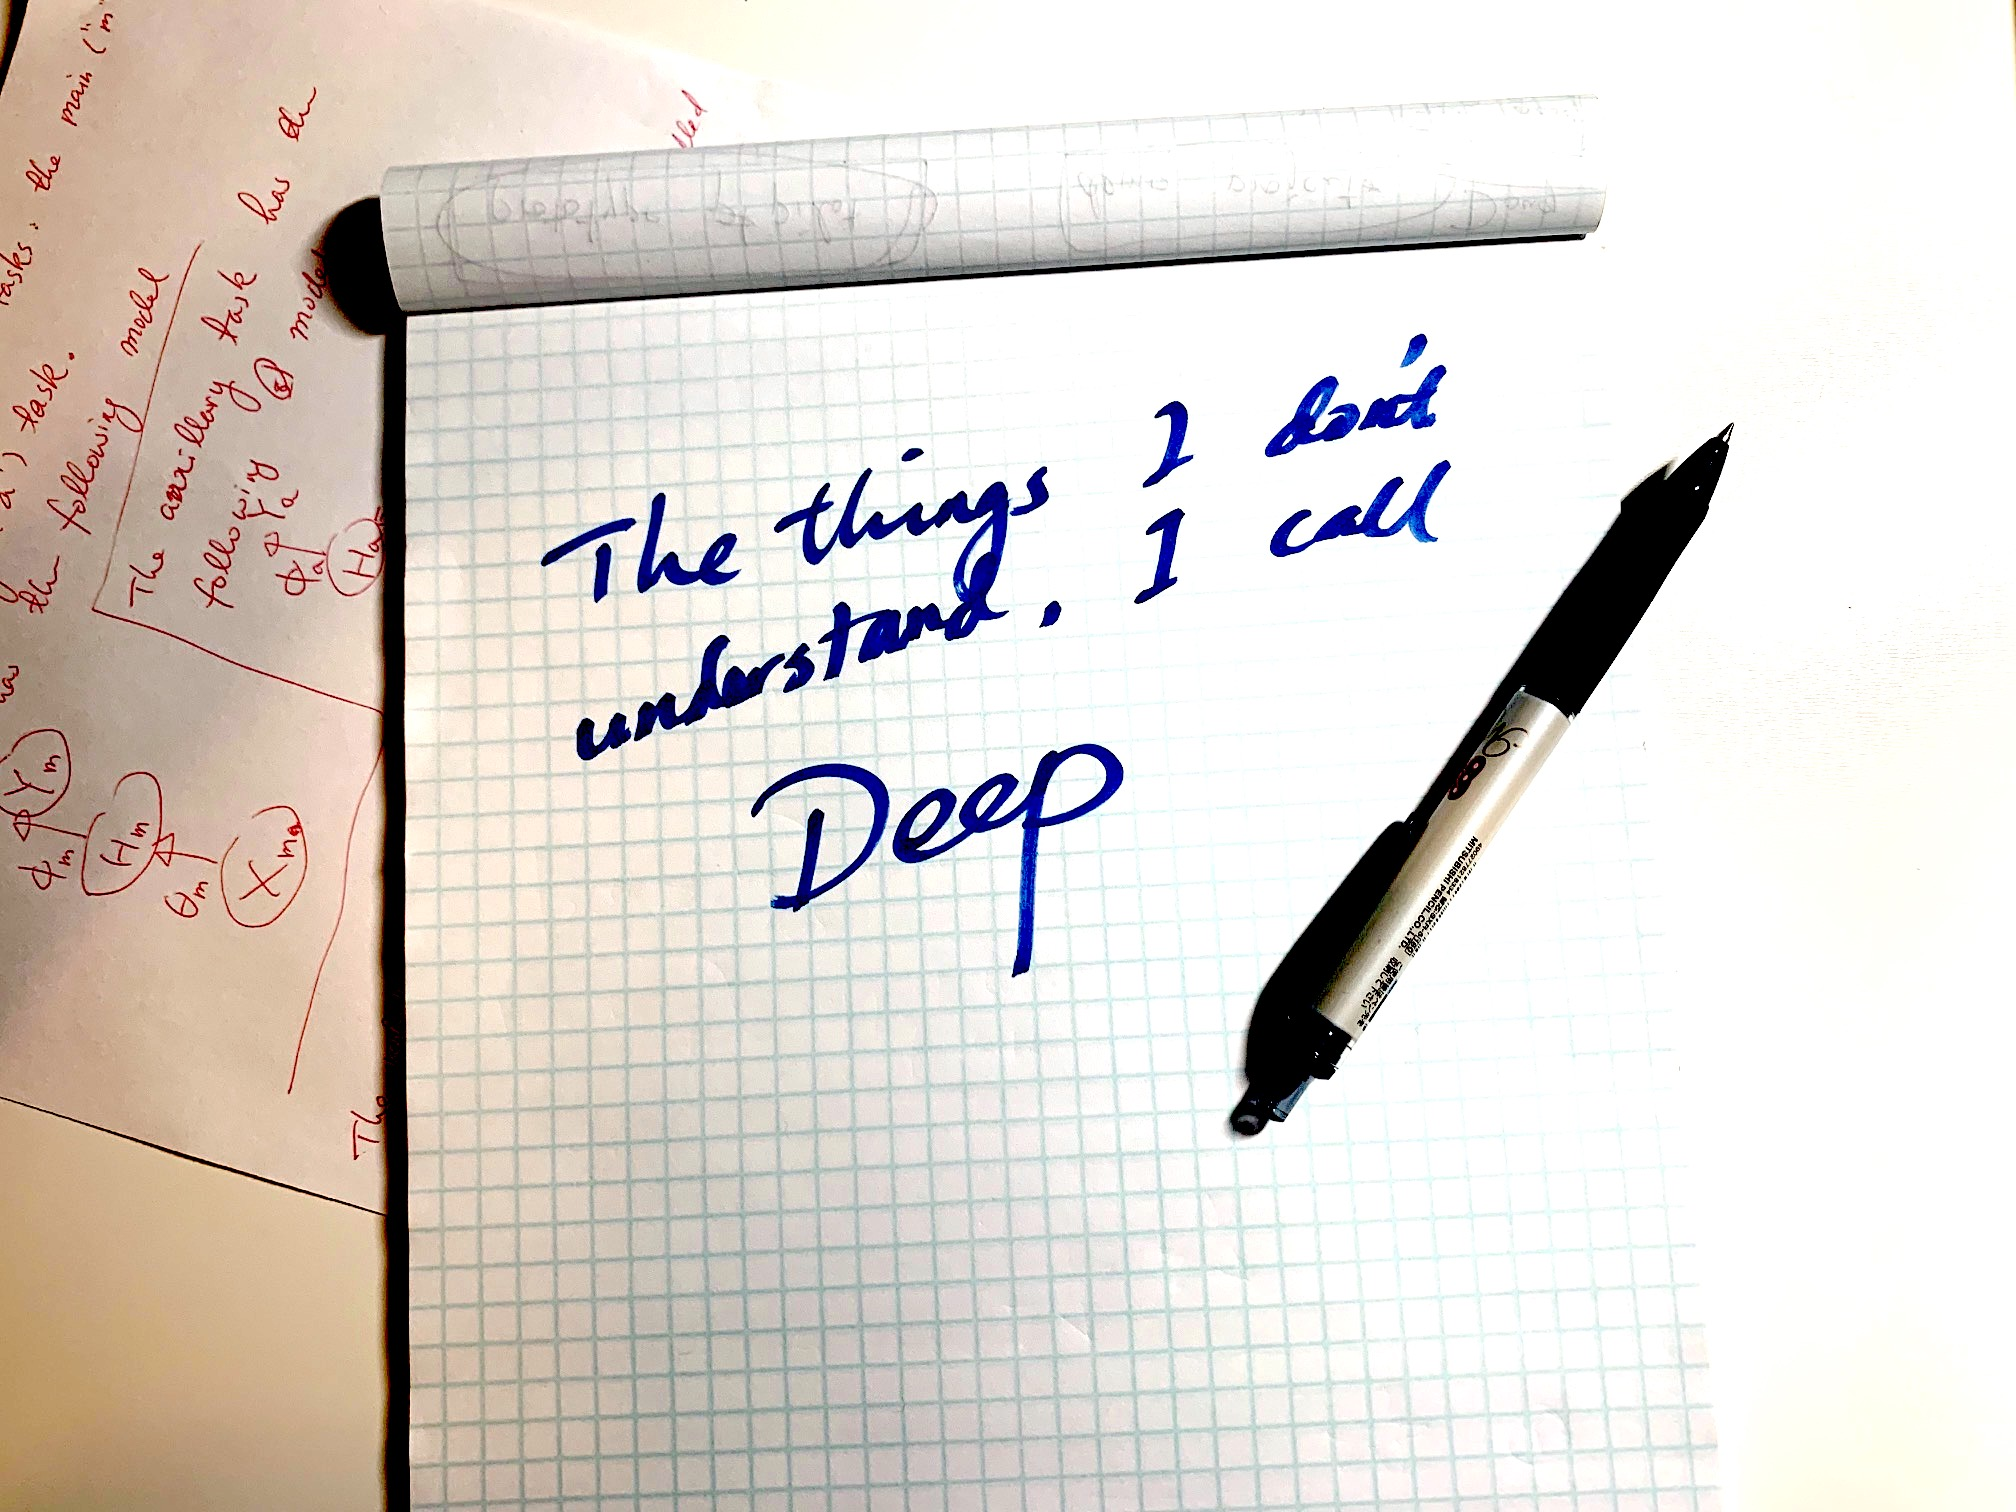
\includegraphics{testImage.jpg}}
\caption{The logo of the course}
\label{fig:logo}
\end{figure}










\section*{Appendix: \LaTeX ing Your Lecture Script}

 Some extra commands are provided by the 
{\tt scribe} package, which may  not be used in the above notes.  
You may open the {\tt scribe.sty} file 
to see this if you have known quite a bit about \LaTeX; alternatively, 
you may open the \LaTeX\ source file of 
this document to see how the following formatted text is generated. 


\begin{definition}
A software is said to be {\em OK} if it is free. 
\end{definition}

\begin{definition}
An OK  software is said to be {\em good} if it is bug-free.
\end{definition}

\begin{definition}
A good software is said to be {\em excellent} if it provides
user-desired functionalities.
\end{definition}



\begin{lemma}
Microsoft WORD is not OK.
\end{lemma}

\Proof :\\
This follows immediately from the definition of OK.
\QED

\begin{lemma}
\LaTeX\ is OK.
\end{lemma}

\Proof :\\
This follows immediately from the definition of ``OK''.
\QED

\begin{proposition}
\LaTeX\ is good.
\end{proposition}

\Proof :\\
This follows immediately from the definition of ``good''.
\QED

\begin{theorem} \LaTeX\ is excellent.
\end{theorem}

\Proof :\\
This follows immediately from the definition of ``excellent''.
\QED

\begin{corollary}
\LaTeX\  is better than Microsoft WORD, with the metric of goodness
defined as above.
\end{corollary}

\Proof :\\
This is a consequence of the first lemma and the above theorem. \QED

\begin{hw}
Remove WINDOWS from your PC, and install Linux. 
\LaTeX\ is there.
\end{hw}

\begin{hw}
Learn \LaTeX.
\end{hw}


\begin{thebibliography}{999}
\bibitem{iid11}
  Clauset, Aaron,
  \textit{A brief primer on probability distributions},
  Santa Fe Institute,
  2011.
\end{thebibliography}

\end{lecture}

\end{document}
